\documentclass{article}
\usepackage[utf8]{inputenc}

\title{Image Processing Library}
\author{Mayank \& Medha}
\date{Jan & Feb 2019}

\usepackage{natbib}
\usepackage{graphicx}

\begin{document}

\maketitle

\section{Introduction}
The task here was to create a \textbf{image processing library} to detect hand written digits. We have to implement different functions and then stitch them together to form a architecture which is capable of detecting hand written digits.
\section{Tasks}
We first implemented some basic function in C++ such as, \textsc{convolution, relu & tanh, softmax and sigmoid function}. We convolved a square matrix with a square kernel, with kernel size less than matrix size. We implemented the function as matrix multiplication and convolution as well. We also implemented the convolution with and without input padding to reduce or maintain the input size. We maintained the inter-dependency of the codes with \textbf{header files and makefile}. We ensured that all the codes were well \textbf{commented, indented and easily readable}. 

There are three files in the source. main.cpp, CLI.cpp and CLI.h which is the header file. To compile and run the program you just need to run the makefile which would create the required object files and link dependencies and produce an executilbe file named main. To test the program simply type -\\
> \textsc{./main inputMatrix.txt matrix\_size inputKernel.txt kernel\_size}

Input files can contain the input in any format, each line contains a single value or all value in a single line separated by commas. The program can handle it. After the program loads, it will print the read `matrix file` and the `kernel file`. After which you can specify operations such as -\\
\\
+ convolution\_withpadding \\
+ convolution\_withpadding\_matrixmult \\
+ convolution\_withoutpadding \\
+ convolution\_withoutpadding\_matrixmult \\
+ relu \\
+ tanh \\
+ sigmoid \\
+ softmax \\
+ avgPooling # takes argument - filterSize & strideSize default strideSize=1 \\
+ maxPooling # takes argument - filterSize & strideSize default strideSize=1 \\

The result is displayed on the screen in a single line and the data is processed sequentially. Here is samples output of the code-\\
\\
> \textsc{\$ ./main matrix.txt kernel.txt}
\\
\\
The input matrix -\\
1 2  3 4 5 1 2 3 4 5 1 2 3 4 5 1 2 3 4 5 1 2 3 4 5\\
The input kernel -\\
1 -2 0 -1 2 -1 1 2 0
\\
\\
> \textsc{convolution\_withpadding}
\\
 2 5 8 11 20 0 2 4 6 14 0 2 4 6 14 0 2 4 6 14 -2 -3 -4 -5 0 \\
 \\
> \textsc{avgpool 3 2}

 3 9.66667 0.333333 4.33333
\\
\\
In subtask 2, we accelerated our program using linear algebra libraries like mkl, openblas and also computed matrix multiplication using pthreads and dealt with synchronization issues. Also we plotted running time of different version of our programs, one with mkl, then with openblas, and pthreads, using gunplot scripts. We made sure that all the different implementation outputs the same result and plotted the timimgs of each.\\
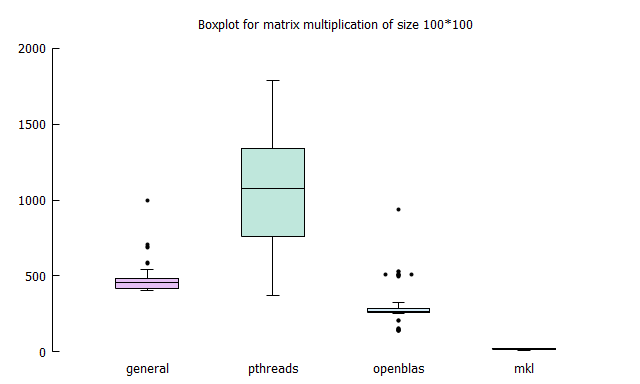
\includegraphics[scale=0.5]{dat100.png}\\
\\
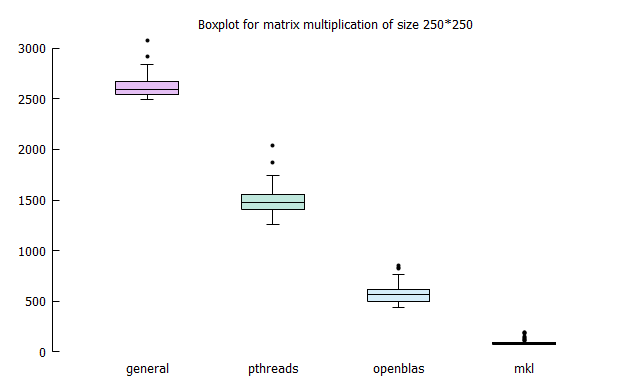
\includegraphics[scale=0.5]{dat250.png}\\
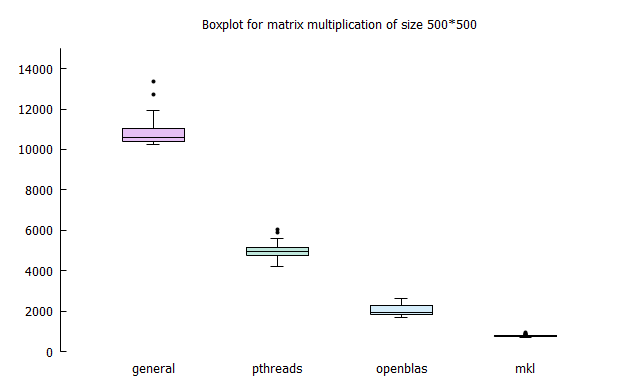
\includegraphics[scale=0.5]{dat500.png}\\
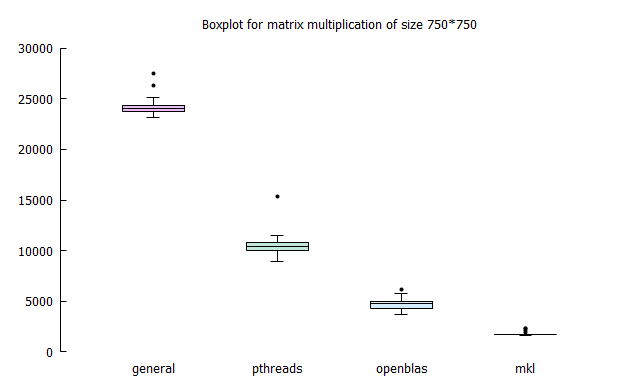
\includegraphics[scale=0.5]{dat750.png}\\
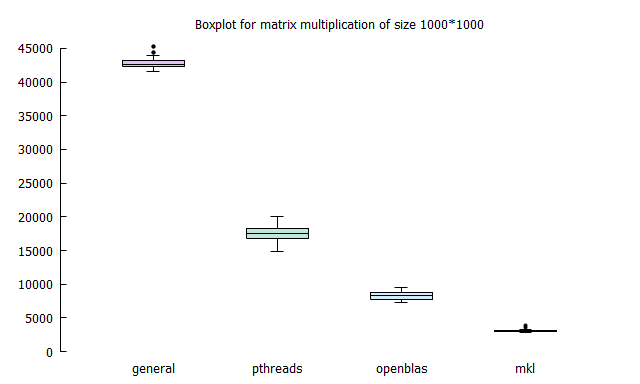
\includegraphics[scale=0.5]{dat1000.png}\\
\\
In the final subtask we implemented the lenet architecture\cite{lenetPrototxt} using our own library. We stitched the above function to map an image (input) to a digit between 0-9 (output label) which constitutes a Convolutional Neural Network (CNN) called LeNet. We tested our implementation on MNIST database of images\cite{mnistdatabase}. The architect, we implemented has two convolutional layers, two pooling layers(maxpool), two fully connected (FC) layers, one relu layer and a softmax layer. We have to take a 28x28 input image and output the top 5 softmax probablity.

To test the program run the lenet executable file with the arguments as normalized float representation of digit in txt format.

\begin{thebibliography}{9}
\bibitem{lenetPrototxt} 
% \textsc{} 
\\\texttt{https://github.com/BVLC/caffe/blob/master/examples/mnist/lenet.prototxt}
 
\bibitem{mnistdatabase}
\textsc{MNIST Database of hand written digits}
Yann LeCun: Courant Institute, NYU;
Corinna Cortes: Google Labs, New York;
Christopher J.C. Burges: Microsoft Research, Redmond;
\\\texttt{http://yann.lecun.com/exdb/mnist/}
\end{thebibliography}
\end{document}
